%%% File encoding: UTF-8
%%% äöüÄÖÜß  <-- keine deutschen Umlaute hier? UTF-faehigen Editor verwenden!

%%% Magic Comments zum Setzen der korrekten Parameter in kompatiblen IDEs
% !TeX encoding = utf8
% !TeX program = pdflatex 
% !TeX spellcheck = de_DE

\documentclass[12pt, letterpaper]{article}

%----------------------------------------------------------------------------------------
%	PACKAGES AND OTHER DOCUMENT CONFIGURATIONS
%----------------------------------------------------------------------------------------

\usepackage[a4paper,left=2.5cm,right=2cm,top=2.5cm,bottom=2.5cm]{geometry}
\usepackage[utf8x]{inputenc}
\usepackage[german]{babel}
\usepackage{graphicx}
\usepackage{caption}
\usepackage{minted} %code
\usepackage{amsmath}
\usepackage[colorinlistoftodos]{todonotes}
\usepackage{fancyhdr}
\usepackage{hyperref}
\usepackage{mathpazo} % Palatino font
\usepackage{float}

%----------------------------------------------------------------------------------------
% SETUP
%----------------------------------------------------------------------------------------

\hypersetup{
    colorlinks,
    citecolor=black,
    filecolor=black,
    linkcolor=black,
    urlcolor=black
}

\pagestyle{fancy}
\fancyhf{}
\rhead{Englisch - Roither}
\lhead{SWK5-WETR}
\rfoot{Seite \thepage}
 
\setminted[]{
	frame=single,
	breaklines,
	samepage=false
} 

\usemintedstyle{csharp}

\graphicspath{ {../pictures/} }

%----------------------------------------------------------------------------------------
% COMMANDS
%----------------------------------------------------------------------------------------

\newcommand{\img}[3] {
\begin{figure}[H]
	\centering
	\includegraphics[width=#3\linewidth]{#1}
	\caption{#2}
\end{figure}
}

 
%----------------------------------------------------------------------------------------
% BEGIN
%----------------------------------------------------------------------------------------

\begin{document}

%----------------------------------------------------------------------------------------
%	TITLE PAGE
%----------------------------------------------------------------------------------------

\begin{titlepage} % Suppresses displaying the page number on the title page and the subsequent page counts as page 1
\newcommand{\HRule}{\rule{\linewidth}{0.5mm}} % Defines a new command for the horizontal lines, change thickness here

\center % Center everything on the page
 
%----------------------------------------------------------------------------------------
%	HEADING SECTIONS
%----------------------------------------------------------------------------------------

\textsc{\LARGE FH Hagenberg}\\[1.5cm] % Name of your university/college
\textsc{\Large Projektarbeit}\\[0.5cm] % Major heading such as course name
%\textsc{\large Minor Heading}\\[0.5cm] % Minor heading such as course title

%----------------------------------------------------------------------------------------
%	TITLE SECTION
%----------------------------------------------------------------------------------------

\HRule \\[0.4cm]
{ \huge \bfseries Weather Tracer - Dokumentation}\\[0.4cm] % Title of your document
\HRule \\[1.5cm]
 
%----------------------------------------------------------------------------------------
%	AUTHOR SECTION
%----------------------------------------------------------------------------------------

\begin{minipage}{0.4\textwidth}
\begin{flushleft} \large
\emph{Autor:}\\
Daniel \textsc{Englisch}\\ % Your name
Andreas \textsc{Roither} % next name
\end{flushleft}
\end{minipage}
~
\begin{minipage}{0.4\textwidth}
\begin{flushright} \large
\emph{Übungsleiter:} \\
Daniel \textsc{Sklenitzka} % Supervisor's Name
\end{flushright}
\end{minipage}\\[2cm]

% If you don't want a supervisor, uncomment the two lines below and remove the section above
%\Large \emph{Author:}\\
%John \textsc{Smith}\\[3cm] % Your name

%----------------------------------------------------------------------------------------
%	DATE SECTION
%----------------------------------------------------------------------------------------

{\large \today}\\[1cm] % Date, change the \today to a set date if you want to be precise
{Version 1.0}\\[2cm]
%----------------------------------------------------------------------------------------
%	LOGO SECTION
%----------------------------------------------------------------------------------------


\includegraphics[scale=0.25]{logo.png}
 
%----------------------------------------------------------------------------------------

\vfill % Fill the rest of the page with whitespace

\end{titlepage}

%----------------------------------------------------------------------------------------

\tableofcontents

\section{Datenbankdesign}

Dieses Projekt wurde mit eines MySQL Datenbank auf Version 5.7.23 realisiert. Es wurden zuerst die geforderten Entitäten aus der Angabe extrahiert und mithilfe eines grafischen Modellierungswerkzeugs namens MySQL Workbench 8\footnote{https://dev.mysql.com/downloads/workbench/} modelliert.

\begin{figure}[H]
\centering
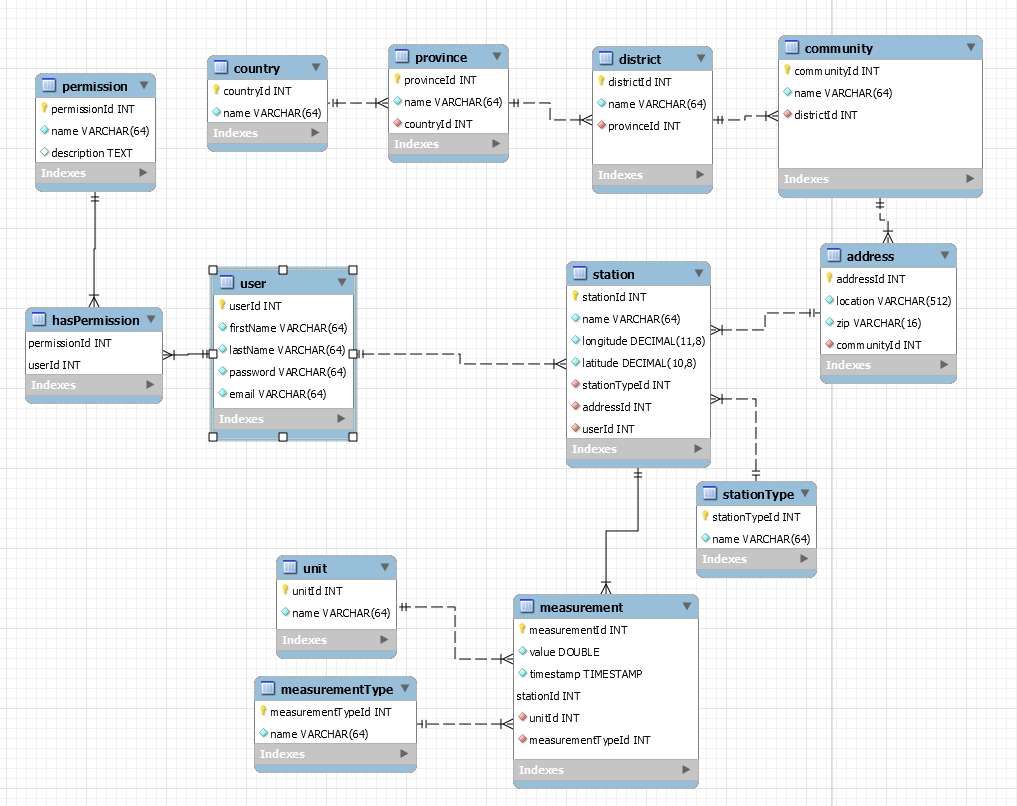
\includegraphics[width=\textwidth]{database.png}
\caption{Datenbankschema des Wetr-Projekts in der ersten Ausbaustufe.}
\label{fig:db}
\end{figure}
\raggedright

Wie in Abbildung \ref{fig:db} zu sehen wird zur Verwaltung des Standortes einer Station eine Reihe von abhängigen Entitäten verwendet. Um die Flexibilität zu erhöhen wurde neben zusätzlich ein \textit{Country} modelliert. In einem \textit{Country} befinden sich \textit{Provinces}, welche Bundesländer darstellen. Jede \textit{Province} wird in mehrere \textit{Districts} unterteilt, ähnlich wie Bezirke. In jedem \textit{District} gibt es mehrere \textit{Communities}, welche mit Gemeinden vergleichbar sind. Als kleinste Entität in dieser Kette gibt es die \textit{Address}, welche einen einfachen String zur Angabe von genaueren Addressdaten (rein zur Anzeige oder falls anderswo benötigt) und eine Zuordnung mittels Postleitzahl enthält.\\
Im Datenbankschema gibt es \textit{User}, welche, falls benötigt, verschiedene \textit{Permissions} zugewiesen haben können. Ein \textit{User} kann mehrere \textit{Stations} betreiben, welche wiederum neben der \textit{Address} auch einen Namen und die Geokoordinaten in Form von Latitide und Longitude gespeichert hat. Der Typ der Station wurde in eine eigene Entität \textit{StationType} ausgelagert.\\
Jede \textit{Station} kann beliebig viele \textit{Measurements} generieren, welche neben den ebenfalls ausgelagerten Entitäten \textit{MeasurementType} und \textit{Unit}, auch einen Zeitstempel und dazugehörigen Messwert besitzen.\\

\subsection{Beispieldaten Generierung}

\subsubsection{Stationen, Addressen und Communities}

Der \textit{Extractor} (befindet sich im extractor Ordner) wurde mit Python\footnote{https://www.python.org/} geschrieben und verwendet die Stationsliste der \textit{Zentralanstalt für Meteorologie und Geodynamik}\footnote{https://www.zamg.ac.at/cms/de/klima/messnetze/wetterstationen}. Die \grqq{}.csv\grqq{} Datei wird vom Extractor eingelesen und für jede \textit{Station} wird eine Insert Anweisung in eine \grqq{}.txt\grqq{} Datei geschrieben. Zusätzlich wird anhand des Längen- und Breitengrades der Ort mit einem geolocator der Aufenthaltsort der Station ermittelt. Anhand dieser Daten werden SQL Anweisungen für die \textit{Community} und \textit{Address} Tabellen erstellt die von der jeweiligen Stationen referenziert werden.

\subsubsection{Messdaten}
Für die erste Ausbaustufe dieses Projekts wurde ein Generator implementiert, der über eine Millionen Messdaten generiert. Diese Messdaten sind jedoch nicht realitätsnahe, sondern haben als Basis den Jahresdurchschnitt in Österreich laut Klimatabelle\footnote{https://www.klimatabelle.info/europa/oesterreich}.
Für eine genauere Beschreibung siehe Abschnitt \ref{sec:generator}.

\subsubsection{Andere Daten}
Die Beispieldaten der restlichen Tabellen wurden per Hand mithilfe vom Internet zusammengestellt. \textit{Provinces}, \textit{Districts} und weiter Standortbezogene Daten sind höchstwarhscheinlich nicht vollständig übernommen worden.
\include{chapters/uml}
\include{chapters/test}
\section{Installationsanleitung}

\subsection{Benötigte Programme und Voraussetzungen}
Für dieses Projekt wird zusätzliche Software benötigt:
\begin{itemize}
\item Docker \footnote{https://www.docker.com/}
\item Visual Studio \footnote{https://visualstudio.microsoft.com/de/}
\item MySql-Connector (optional, nur falls notwendig) \footnote{https://dev.mysql.com/get/Downloads/Connector-Net/mysql-connector-net-8.0.13.msi}
\end{itemize}
\raggedright

Um die Datenbank zu erstellen muss Docker gestartet sein. Die Datenbank kann mit dem \textit{Powershell-Script} \grqq{}run.ps1 \grqq{} automatisch generiert werden.
Falls dieses Script wegen fehlender Berechtigungen nicht ausgeführt werden kann, muss eine \textit{Shell} (Git-Bash oder ähnliches) im Ordner mit der Docker Compose Datei \grqq{}docker-compose.yaml \grqq{} geöffnet und folgenden Befehle nacheinander ausgeführt werden:
\begin{minted}{dockerfile}
docker stop $(docker ps -a -q)
docker rm $(docker ps -a -q)
docker-compose up --build --force-recreate
\end{minted}

\subsection{Datenbank}
Für die Datenbank muss die SQL Datei \grqq{}create-wetr.sql \grqq{} im Ordner sql/Create ausgeführt werden. Falls das Unit Testing auch ausgeführt werden soll, wird die zweite SQL Datei \grqq{}create\textunderscore wetr-unit.testing.sql \grqq{} auch benötigt.
\newline\newline
Für die Füllung der Datenbank kann die SQL Datei \grqq{}InsertEverythingWithoutMeasurement.sql\grqq{} verwendet werden. Für die Measurement Daten muss spezieller vorgegangen werden dadurch kann aber die Insert Zeit drastisch verringert werden:
\begin{itemize}
\item Wetr.Generator.exe im Ordner sql/Insert starten
\item http://localhost:8080/ im Browser aufmachen \newline (phpMyAdmin sollte starten)
\item Benutzer: root Passwort: 0c1cd84e
\item Datenbank wetr auswählen
\item Zum SQL Tab wechseln
\item Die nachfolgenden SQL Anweisungen eingeben und ausführen
\end{itemize}
\newpage
\begin{minted}{sql}
LOAD DATA LOCAL INFILE "/tmp/sql/insert/measurementsDownfall.bulk" INTO TABLE measurement
FIELDS TERMINATED BY ', ' ENCLOSED BY "'"
LINES TERMINATED BY '\r\n';

LOAD DATA LOCAL INFILE "/tmp/sql/insert/measurementsHumidity.bulk" INTO TABLE measurement
FIELDS TERMINATED BY ', ' ENCLOSED BY "'"
LINES TERMINATED BY '\r\n';

LOAD DATA LOCAL INFILE "/tmp/sql/insert/measurementsTemperature.bulk" INTO TABLE measurement
FIELDS TERMINATED BY ', ' ENCLOSED BY "'"
LINES TERMINATED BY '\r\n';

LOAD DATA LOCAL INFILE "/tmp/sql/insert/measurementsWind.bulk" INTO TABLE measurement
FIELDS TERMINATED BY ', ' ENCLOSED BY "'"
LINES TERMINATED BY '\r\n';

LOAD DATA LOCAL INFILE "/tmp/sql/insert/measurementsWindDirection.bulk" INTO TABLE measurement
FIELDS TERMINATED BY ', ' ENCLOSED BY "'"
LINES TERMINATED BY '\r\n';

LOAD DATA LOCAL INFILE "/tmp/sql/insert/measurementsPreassure.bulk" INTO TABLE measurement
FIELDS TERMINATED BY ', ' ENCLOSED BY "'"
LINES TERMINATED BY '\r\n';
\end{minted}


\end{document}
